\documentclass[11pt]{article}
\usepackage[a4paper,margin=25mm]{geometry}
\usepackage[T1]{fontenc}
\usepackage[utf8]{inputenc}
\usepackage{lmodern}
\usepackage{graphicx}
\usepackage{booktabs}
\usepackage{amsmath}
\usepackage{xspace}
\usepackage{hyperref}
\graphicspath{{../fullsim_analysis/results/2026-10_ambient/study/}}
\newcommand{\us}{\textmu s\xspace}
\newcommand{\Na}{\ensuremath{{}^{22}\mathrm{Na}}\xspace}
\newcommand{\Vov}{\ensuremath{V_{\rm ov}}\xspace}
\newcommand{\csitl}{CsI(Tl)\xspace}

\title{BGO and \csitl crystals read by 64 SiPMs at room temperature:\\
a simulation of three readouts}
\author{J.\,J.~Gómez-Cadenas}
\date{18 October 2026}

\begin{document}
\maketitle

\begin{abstract}
We simulate the response of two $48 \times 48$~mm$^2$ scintillating
crystals, BGO and \csitl, read through optical grease by an $8 \times 8$
array of SiPMs at room temperature and irradiated by a \Na source. The
simulation follows each decay from the gamma interactions in the crystal to
the charge recorded by three readouts: the Citiroc~1A and the Radioroc2,
two ASICs that shape the signal and store its maximum, and the CAEN DT2745,
a waveform digitiser whose records are integrated offline. For each of the
six combinations of crystal and readout we determine the trigger, the
calibration of the SiPM gain from their dark counts, the energy spectrum,
the energy resolution at 511~keV and the number of photoelectrons. The
crystals produce 3885 (BGO) and 27\,600 (\csitl) photons per 511~keV
deposit, of which 84\% reach the SiPMs and 41\% (BGO) or 32 to 35\%
(\csitl) become photoelectrons. The energy resolution is 10.1, 9.1 and
8.5\% FWHM for BGO and 7.4, 6.1 and 6.1\% for \csitl with the Citiroc, the
digitiser and the Radioroc2 respectively. The intrinsic resolution of the
crystals, taken as 5\%, and the statistics of the photoelectrons dominate
the width; the readout adds a contribution that is largest for the
Citiroc, whose short shaping keeps a small and fluctuating fraction of the
light, and smallest for the Radioroc2. The dark counts of the SiPMs at room
temperature, about 4~MHz per channel, prevent the calibration of the
Radioroc2 at its long shaping time and that of the digitiser at unit gain,
and impose the procedures described here.
\end{abstract}

\tableofcontents

\section{Introduction}

The CRYSP project studies scintillating crystals read by arrays of SiPMs for
the detection of 511~keV gammas, with the energy and the position of the
interaction as the quantities of interest. The measurements of the coming
weeks use two crystals, BGO and \csitl, an array of 64 SiPMs and three
readouts: the CAEN DT2745 digitiser, which records the waveform of each
channel, and two ASICs from Weeroc, the Citiroc~1A and the Radioroc2, which
shape the signal of each channel and store its maximum. The three readouts
answer the same questions in different ways and with different
limitations, and the measurements alone cannot separate the properties of
the crystal from those of the readout.

This note presents the simulation of the six combinations of crystal and
readout at room temperature, with the operating conditions that the
measurements will use. For each of them it establishes how the
acquisition is triggered, how the gain of the SiPMs is calibrated, which
energy spectrum is recorded, which energy resolution is reached at
511~keV and how many of the emitted photons become photoelectrons and
recorded charge. The comparison of the six cases identifies the
contributions to the energy resolution and their origin. The position of
the interaction will be the subject of a separate note.

Section~\ref{sec:setup} describes the set-up and Section~\ref{sec:sim} the
simulation. Section~\ref{sec:conditions} gives the operating conditions of
the six cases and Section~\ref{sec:analysis} the analysis common to all of
them. Sections~\ref{sec:bgo} and~\ref{sec:csi} present the results for
each crystal and readout, Section~\ref{sec:comparison} compares them and
Section~\ref{sec:conclusions} concludes.

\section{The set-up}
\label{sec:setup}

Both crystals have a face of $48 \times 48$~mm$^2$; the BGO crystal is
22.4~mm and the \csitl crystal 37.2~mm deep (Figure~\ref{fig:geometry}).
They are wrapped in PTFE tape, with an air gap between the crystal and the
tape, on every face except the one coupled to the SiPMs. The coupling is a
layer of optical grease of refractive index 1.42 followed by the silicone
resin window of the SiPM tiles, of index 1.57. The SiPMs are Hamamatsu
S14161-6050HS-04 tiles, each holding $4 \times 4$ channels of
$6 \times 6$~mm$^2$ at a pitch of 6.2~mm; four tiles form the
$8 \times 8$ array, which covers $50 \times 50$~mm$^2$ and therefore
overhangs the crystal by 1~mm on each side. A \Na source sits on the axis
of the crystal, 30~mm from the face opposite to the SiPMs. Each decay emits
a 1275~keV gamma and, in 90\% of the decays, a pair of back-to-back
511~keV gammas from the annihilation of the positron.

\begin{figure}[htbp]
\centering
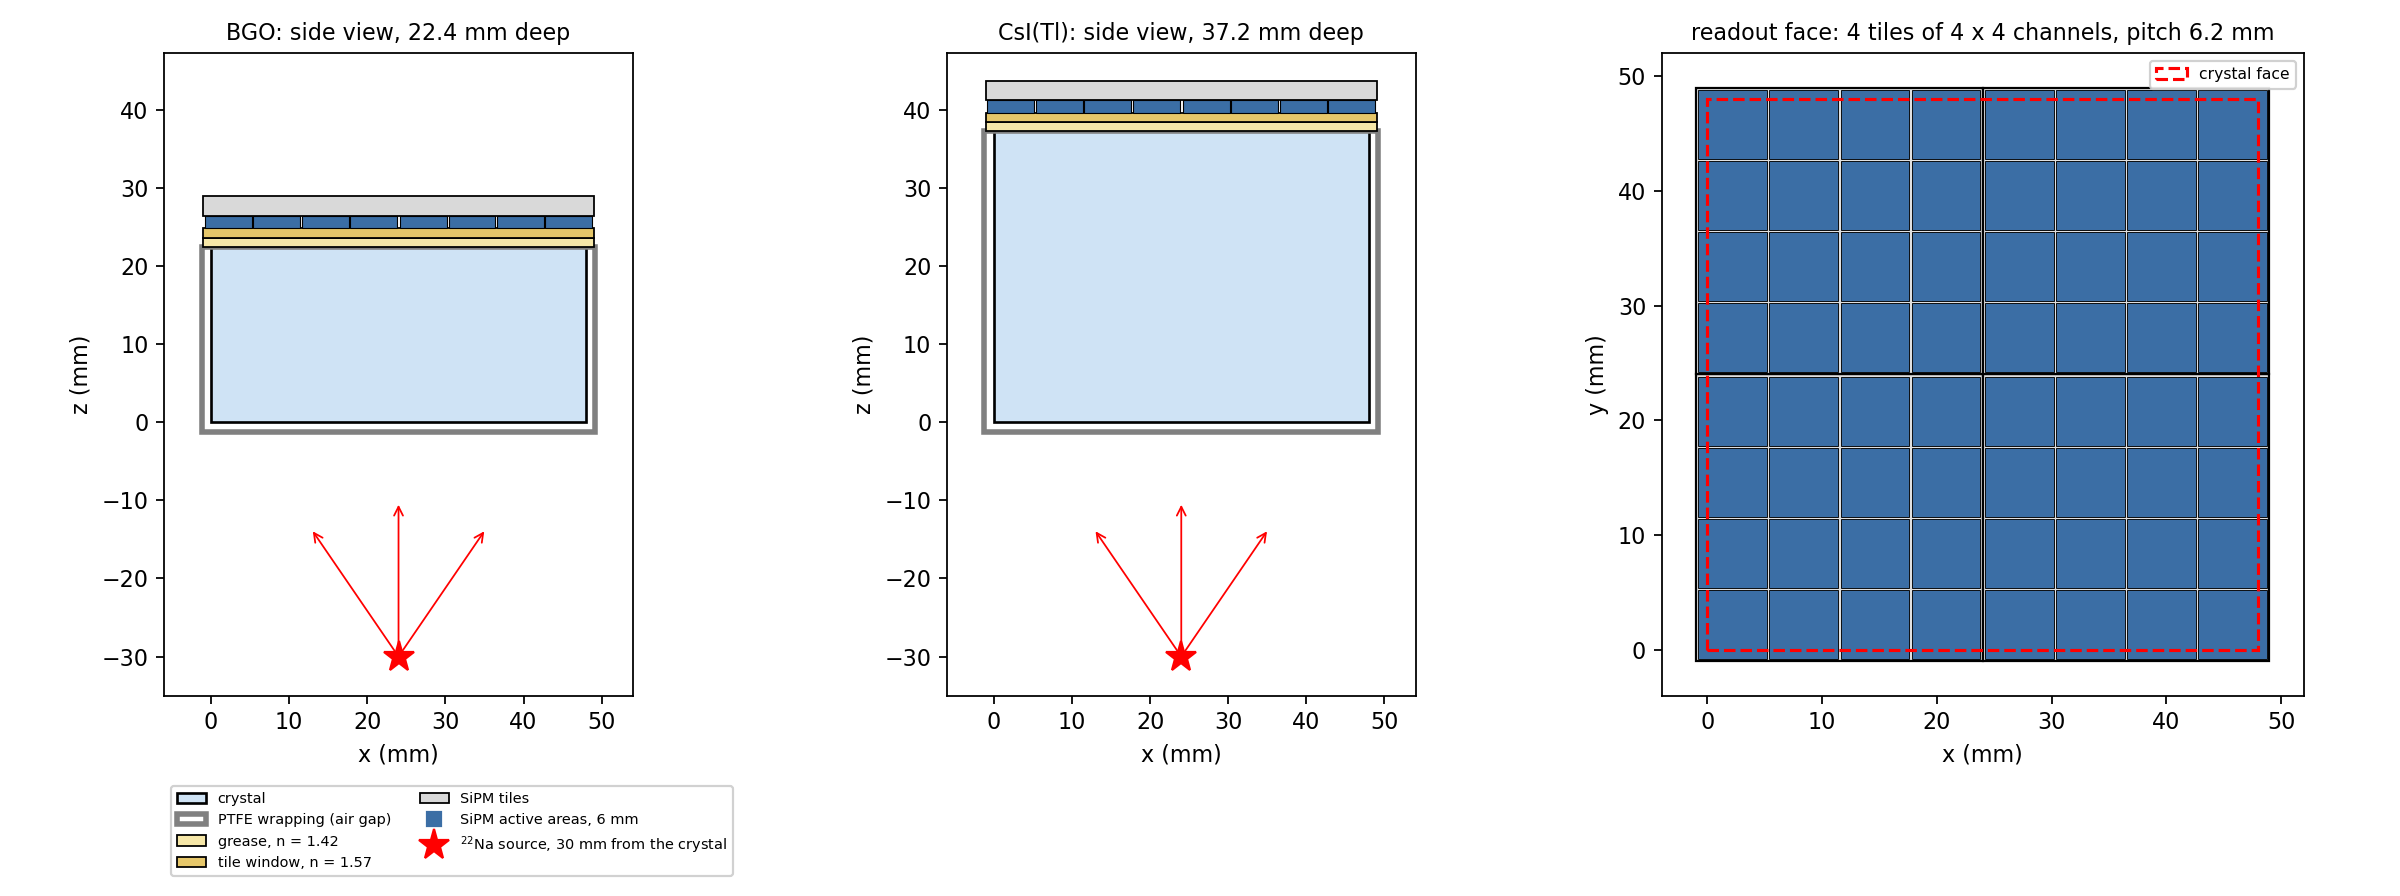
\includegraphics[width=\textwidth]{geometry.png}
\caption{The simulated geometry. Side views of the two crystals with the
wrapping, the grease, the window and the SiPM tiles (the coupling layers
are drawn thicker than they are), and the source; face view of the 64
active areas, grouped in four tiles, with the outline of the crystal.}
\label{fig:geometry}
\end{figure}

\section{The simulation}
\label{sec:sim}

The simulation proceeds in three stages, each writing a file that the next
one reads. The first stage generates the \Na decays, transports the gammas
through the crystal (photoelectric absorption and Compton scattering,
with pair production absorbed locally) and converts each energy deposit into scintillation photons.
The number of photons is the light yield of the crystal, 7600 photons per
MeV for BGO and 54\,000 for \csitl at room temperature, times the
deposited energy, multiplied by one Gaussian factor per decay that
represents the intrinsic resolution of the crystal: 5\% FWHM at 511~keV for
both crystals, scaling as the inverse square root of the energy. The
photons are emitted with the time distribution of the crystal, two components of
300~ns (90\%) and 60~ns (10\%) for BGO and of 730~ns
(64\%) and 3340~ns (36\%) for \csitl, at the wavelength of the emission
maximum, 480~nm for BGO and 550~nm for \csitl. The photons are then transported through the crystal,
its surfaces, the wrapping and the coupling layers until they are absorbed
or reach the active area of a SiPM; the stage records every photon that
arrives there, with its channel, time and wavelength.

The second stage applies the response of the SiPMs. Each recorded photon
produces a photoelectron with the photon detection efficiency of the
device at its wavelength and at the overvoltage of the run, the excess of
the bias voltage over the breakdown voltage. Each photoelectron fires a
cell, which may in turn fire neighbouring cells by optical crosstalk and
produce delayed afterpulses; independently, thermal dark counts fire cells
at random times with the same companions. All these depend on the
overvoltage; Table~\ref{tab:conditions} gives their values. We call
\emph{fired cells} the sum of photoelectrons, crosstalk and afterpulses
produced by the scintillation light, and use the charge of one fired cell,
the gain of the SiPM, as the unit of charge: a recorded charge divided by
it is expressed in \emph{photoelectron equivalents}. The gain of each
channel differs from the nominal one by a Gaussian factor of 5\% rms.

The third stage applies the readout to the train of fired cells of each
channel. For the Citiroc and the Radioroc2 the train is shaped by a
semi-Gaussian filter of order two with the peaking time of the chip,
noise is added, a trigger is formed from the discriminators of the chip,
and a peak detector stores the maximum of the shaped signal of every
channel from the trigger until the \emph{hold}, a fixed delay after the
trigger, before the conversion by an ADC. For the digitiser, the charge
that the offline analysis integrates over a window, minus the baseline
measured before it, is computed directly from the times of the fired
cells, and the trigger is formed from the sampled amplitude of each
channel with its noise. The three stages and the parameters of each model
are described in the design document of the simulation.

\section{Operating conditions}
\label{sec:conditions}

The operating conditions are those planned for the measurements and are
the best compromise found by the simulation for each readout
(Table~\ref{tab:conditions}). The overvoltage of the SiPMs is 3~V for both
ASICs with BGO; with \csitl, whose light is seven times more abundant, it
is lowered to keep the brightest channel within the range of the chip:
to 2.7~V for the Citiroc, whose input saturates at 400~pC, and to 2.0~V for
the Radioroc2, whose low-gain path saturates at 2000 photoelectrons of
unit gain $10^6$. The digitiser operates at 5~V, the setting used so far
on the bench, at a gain of 4, which places one photoelectron at 64~ADC
counts against a noise of 4~counts per sample. The Citiroc shapes the
signal with its longest peaking time, 87.5~ns; the Radioroc2 with its
longest, 1.8~\us, on both its high-gain and low-gain paths, and the
energy is read from the low-gain path. The digitiser integrates over
1~\us for BGO and 3~\us for \csitl, starting 50~ns before the trigger,
with a baseline measured over the 900~ns before the integration window;
these values minimise the energy resolution in a scan of the window.

\begin{table}[htbp]
\centering
\small
\caption{Operating conditions of the six cases. The detection efficiency
is the photon detection efficiency at the peak of its spectral curve; the
dark-count rate is per channel; the window is the hold of the ASICs and
the integration window of the digitiser. Thresholds in photoelectron
equivalents.}
\label{tab:conditions}
\begin{tabular}{l ccc ccc}
\toprule
 & \multicolumn{3}{c}{BGO} & \multicolumn{3}{c}{\csitl} \\
 & Citiroc & DT2745 & Radioroc2 & Citiroc & DT2745 & Radioroc2 \\
\midrule
overvoltage (V) & 3.0 & 5.0 & 3.0 & 2.7 & 5.0 & 2.0 \\
SiPM gain ($10^6$) & 2.8 & 4.7 & 2.8 & 2.5 & 4.7 & 1.9 \\
detection efficiency & 0.52 & 0.54 & 0.52 & 0.50 & 0.54 & 0.41 \\
crosstalk probability & 0.088 & 0.195 & 0.088 & 0.070 & 0.195 & 0.041 \\
dark-count rate (MHz) & 4.3 & 4.4 & 4.3 & 4.1 & 4.4 & 3.3 \\
shaping (ns) & 87.5 & --- & 1800 & 87.5 & --- & 1800 \\
window (ns) & 300 & 1000 & 3560 & 500 & 3000 & 3560 \\
trigger & single, 8 & two, 7.5 & charge, 40 & single, 7 & two, 7.5 & charge, 40 \\
\bottomrule
\end{tabular}
\end{table}

The trigger differs between the readouts. The Citiroc triggers when one
channel crosses the threshold of its fast discriminator, which follows a
shaper of 15~ns. The digitiser triggers when two channels cross the
threshold within 100~ns, a coincidence that we call a majority of two.
The Radioroc2 triggers on its charge discriminator, which reads the
low-gain shaped signal of each channel. In each case the threshold is the
lowest one at which every 511~keV photopeak event triggers (an efficiency
of at least 0.995) while the dark counts, alone, trigger less than once per
millisecond. At room temperature this second condition is the restrictive
one: a dark count with three or four crosstalk companions occurs in some
channel in most microseconds, and thresholds of a few photoelectrons
trigger on it.

\section{Analysis}
\label{sec:analysis}

The analysis treats the simulated files as it will treat the measured ones,
and uses the record of the simulation only to select the events and to
follow the light from the crystal to the readout.

\emph{Calibration.} The gain of each channel is measured on the dark
counts, recorded without source. For the ASICs, each channel triggers on
its own discriminator at half a photoelectron and its high-gain signal is
held at the peaking time after the trigger, which records the amplitude of
the dark pulse that triggered; only the channels whose discriminator fired
within 2~ns of the trigger enter the spectrum, since the others are held
at a random phase of their signal. For the digitiser, every record
contains tens of dark pulses per channel; the waveform is filtered with
the sampled pulse of one fired cell (a matched filter) after subtracting
the mean of the four preceding samples, and the local maxima of the
filtered waveform are the pulse amplitudes. In both cases the position of
the one-photoelectron peak of each channel, from a Gaussian fit, is its
gain.

\emph{Pedestal.} The peak detectors of the ASICs store, in a channel that
receives no light, the largest dark pulse or noise excursion within the
hold, never zero. This pedestal is measured on events with no energy
deposit read with a random trigger, and subtracted channel by channel. It
amounts to 1.5 photoelectron equivalents per channel for the Citiroc and
9 to 12 for the Radioroc2, whose hold is ten times longer; the
digitiser, whose baseline is subtracted, has none.

\emph{Energy.} The energy of an event is the sum of the 64 channels. A
straight line through the positions of the 511 and 1275~keV peaks
converts it into keV; this calibration absorbs the residual offset left
by the pedestal, which is not exactly additive, since in a channel that
receives light a dark pulse changes the stored maximum only when it falls
on top of the signal. The 511~keV peak is fitted with a Gaussian on a
linear background, and the energy resolution is its FWHM divided by its
position.

\emph{Light.} The events in which one 511~keV gamma deposits its full
energy in the crystal, without any deposit of the 1275~keV gamma, are
selected from the record of the simulation; they number between 7000 and
52\,000 per case. On these events we count the photons emitted, the
photons that reach the active areas of the SiPMs, the photoelectrons and
the fired cells, the last two from a replay of the SiPM response without
dark counts, and we take the recorded charge at 511~keV in photoelectron
equivalents from the energy calibration. The ratios between consecutive
quantities are the collection efficiency of the crystal and its coupling,
the detection efficiency at the emission wavelength, and the
fraction of the photoelectrons that the readout records.

\emph{Resolution.} On the same events, the relative width of each quantity
(half the interval between its 16th and 84th percentiles divided by its
median, multiplied by 2.355 to compare with a FWHM) separates the
contributions to the energy resolution. The width of the number of
photoelectrons contains the intrinsic resolution of the crystal and the
statistics of the light collection and detection; the difference in
quadrature with the intrinsic 5\% is the statistical contribution. The
difference in quadrature between the widths of the fired cells and of the
photoelectrons is the contribution of crosstalk and afterpulses; that
between the recorded energy and the fired cells is the contribution of the
readout, which includes the dark counts, the electronic noise, the
fluctuation of the fraction of the light that the shaping keeps and the
pedestal.

\section{BGO}
\label{sec:bgo}

A 511~keV deposit in BGO emits 3885 photons, of which 3254 (84\%) reach the
SiPMs and 1585 become photoelectrons at 3~V, 1634 at 5~V. The width of the
number of photoelectrons is 7.7\% FWHM, the intrinsic 5\% and a
statistical term of 5.9\%, the value expected from 1585 photoelectrons.

\subsection{Citiroc 1A}

The single-channel threshold of 8 photoelectron equivalents triggers on
every 511~keV event and on 98.5\% of the deposits between 200 and
300~keV, while the dark counts trigger at 0.3~kHz
(Figure~\ref{fig:bgo_citiroc}). The single-photoelectron spectrum shows
clean peaks; the fitted gain is 0.885 of the true one, because the hold at
the peaking time after the discriminator falls slightly after the maximum,
a factor common to all channels that the energy calibration absorbs. The
fitted gains follow the true ones channel by channel to 1.4\%, against the
5\% spread of the gains; in 6 channels of 64 the fit takes the
two-photoelectron peak and must be repeated. The shaping of 87.5~ns keeps
a small part of a 300~ns light pulse: the recorded charge at 511~keV is
726 photoelectron equivalents, 0.46 of the photoelectrons. The energy
resolution is 10.1\% FWHM. The readout contributes 5.9\%, as much as the
statistics: the fraction of the light that a short shaping keeps depends
on the times of arrival of the photoelectrons and fluctuates from event to
event. The ratio of the 1275 and 511~keV peak positions is 2.48 before
calibration, close to the 2.50 of a linear response.

\begin{figure}[htbp]
\centering
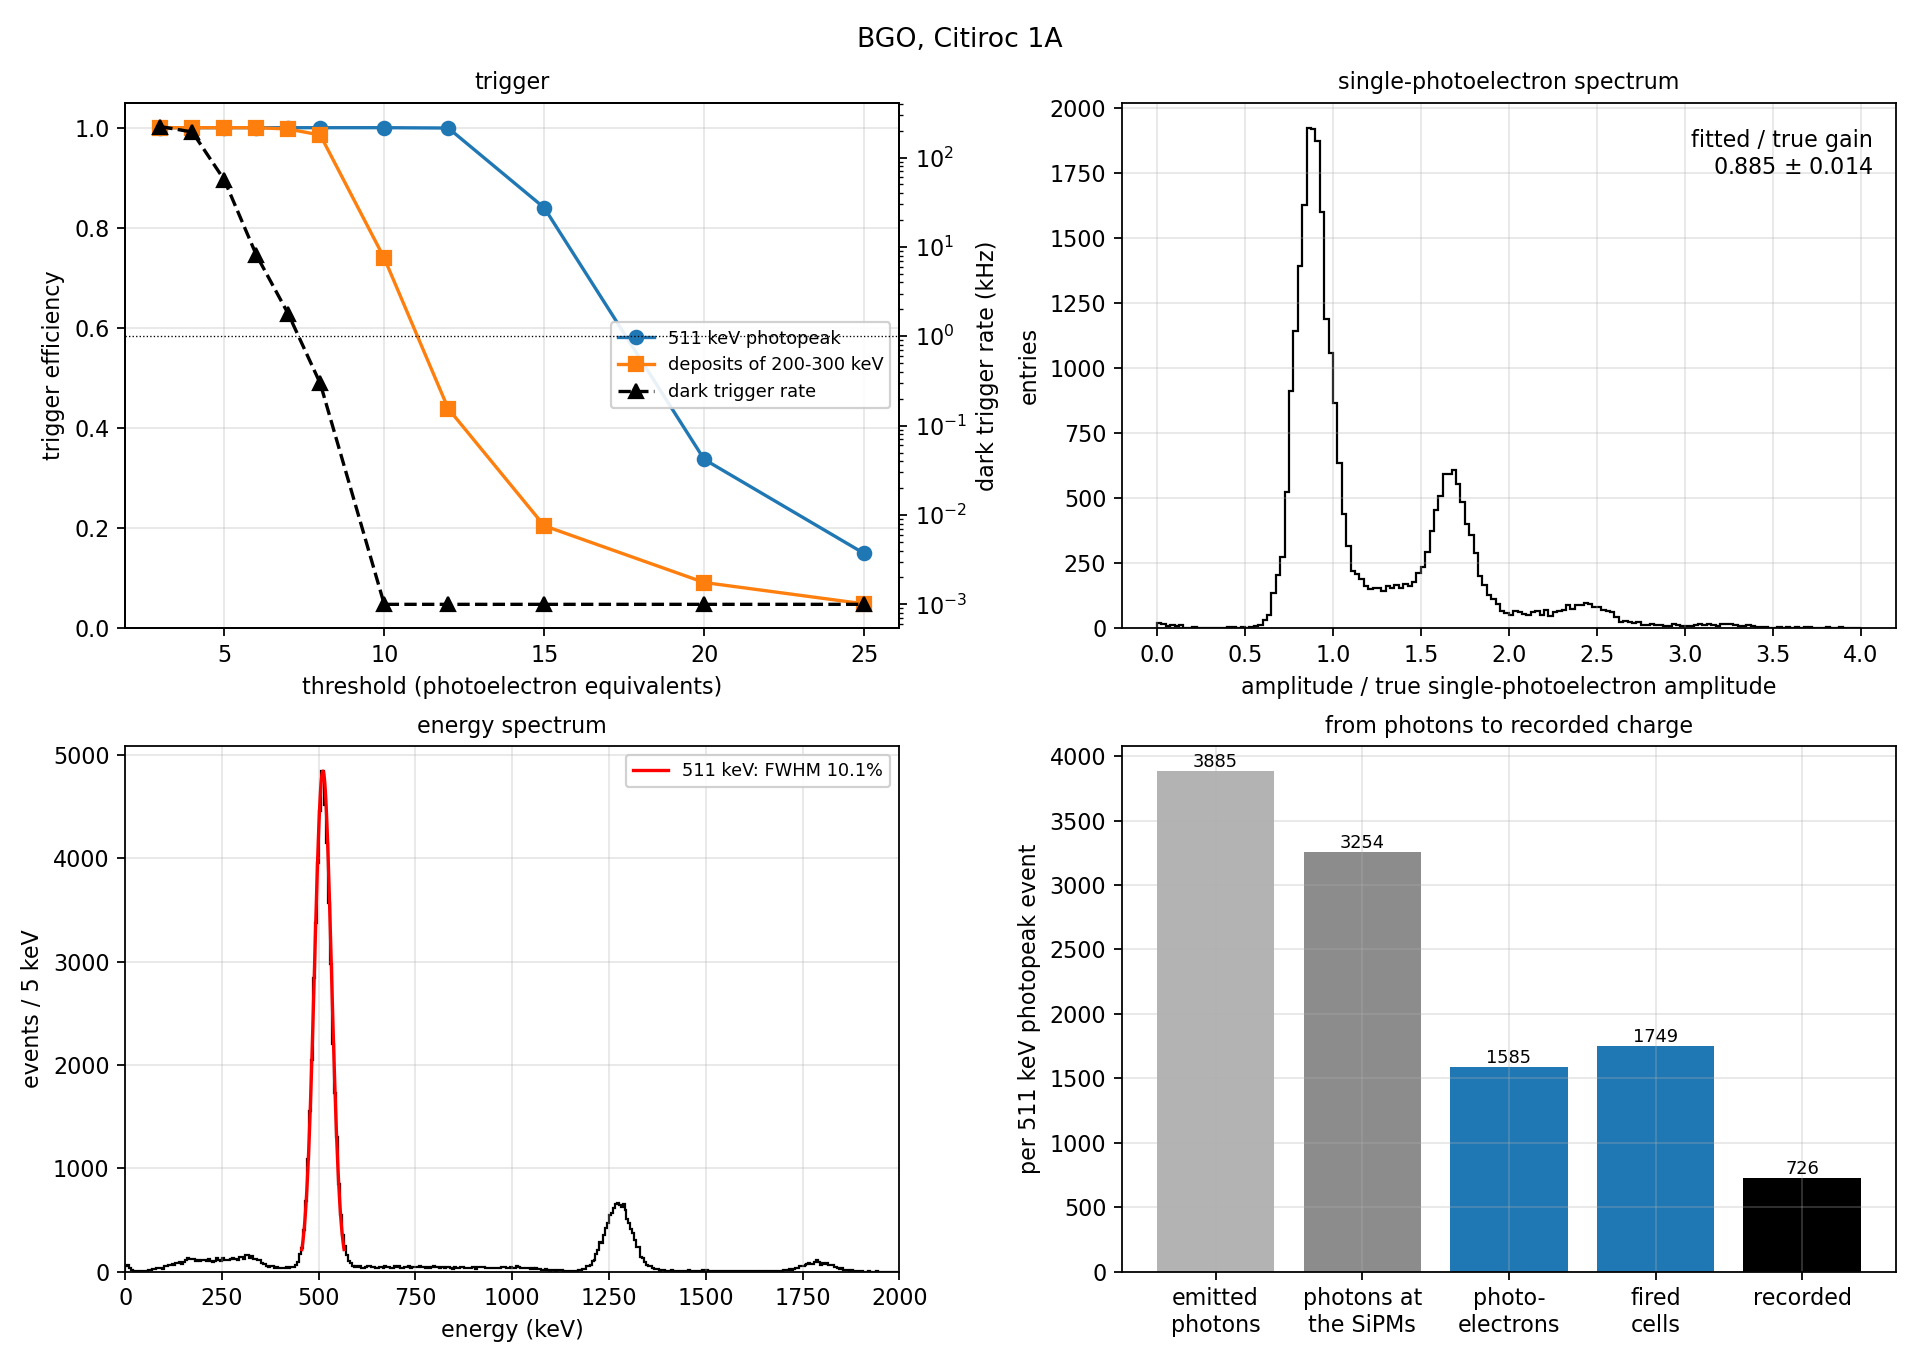
\includegraphics[width=\textwidth]{case_bgo_citiroc.png}
\caption{BGO read by the Citiroc~1A. Top left: trigger efficiency for the
511~keV photopeak and for deposits of 200 to 300~keV, and dark trigger
rate, against the threshold; rates below the sensitivity of the sample
are drawn at $10^{-3}$~kHz. Top right: single-photoelectron spectrum of the
dark counts, all channels, each normalised to its true gain. Bottom left:
calibrated energy spectrum with the fit of the 511~keV peak. Bottom right:
photons emitted, photons at the SiPMs, photoelectrons, fired cells and
recorded charge per 511~keV photopeak event.}
\label{fig:bgo_citiroc}
\end{figure}

\subsection{DT2745 digitiser}

The threshold of 480~ADC counts, 7.5 photoelectrons, with a majority of
two triggers on every 511~keV event and on 98.6\% of the deposits between
200 and 300~keV; no event without deposit triggers in the sample, which
bounds the dark trigger rate below 0.3~kHz (Figure~\ref{fig:bgo_dig}). At
gain 4 the matched filter separates the single-photoelectron peaks
cleanly; the fitted gain is 0.981 of the true one with a spread of 0.1\%
between channels, and the one-photoelectron peak has a width of 6\% of its
position. The integration window of 1~\us records the whole light pulse,
so that the recorded charge, 1966 photoelectron equivalents, exceeds the
1634 photoelectrons by the crosstalk (19.5\% at 5~V) and the afterpulses.
The energy resolution is 9.1\% FWHM. Crosstalk and afterpulses contribute
2.9\%, and the readout 4.3\%: the integration window collects 280 dark
counts on average over the 64 channels, with their crosstalk, and their
fluctuation adds to the width. The ratio of the peak positions is 2.49.

\begin{figure}[htbp]
\centering
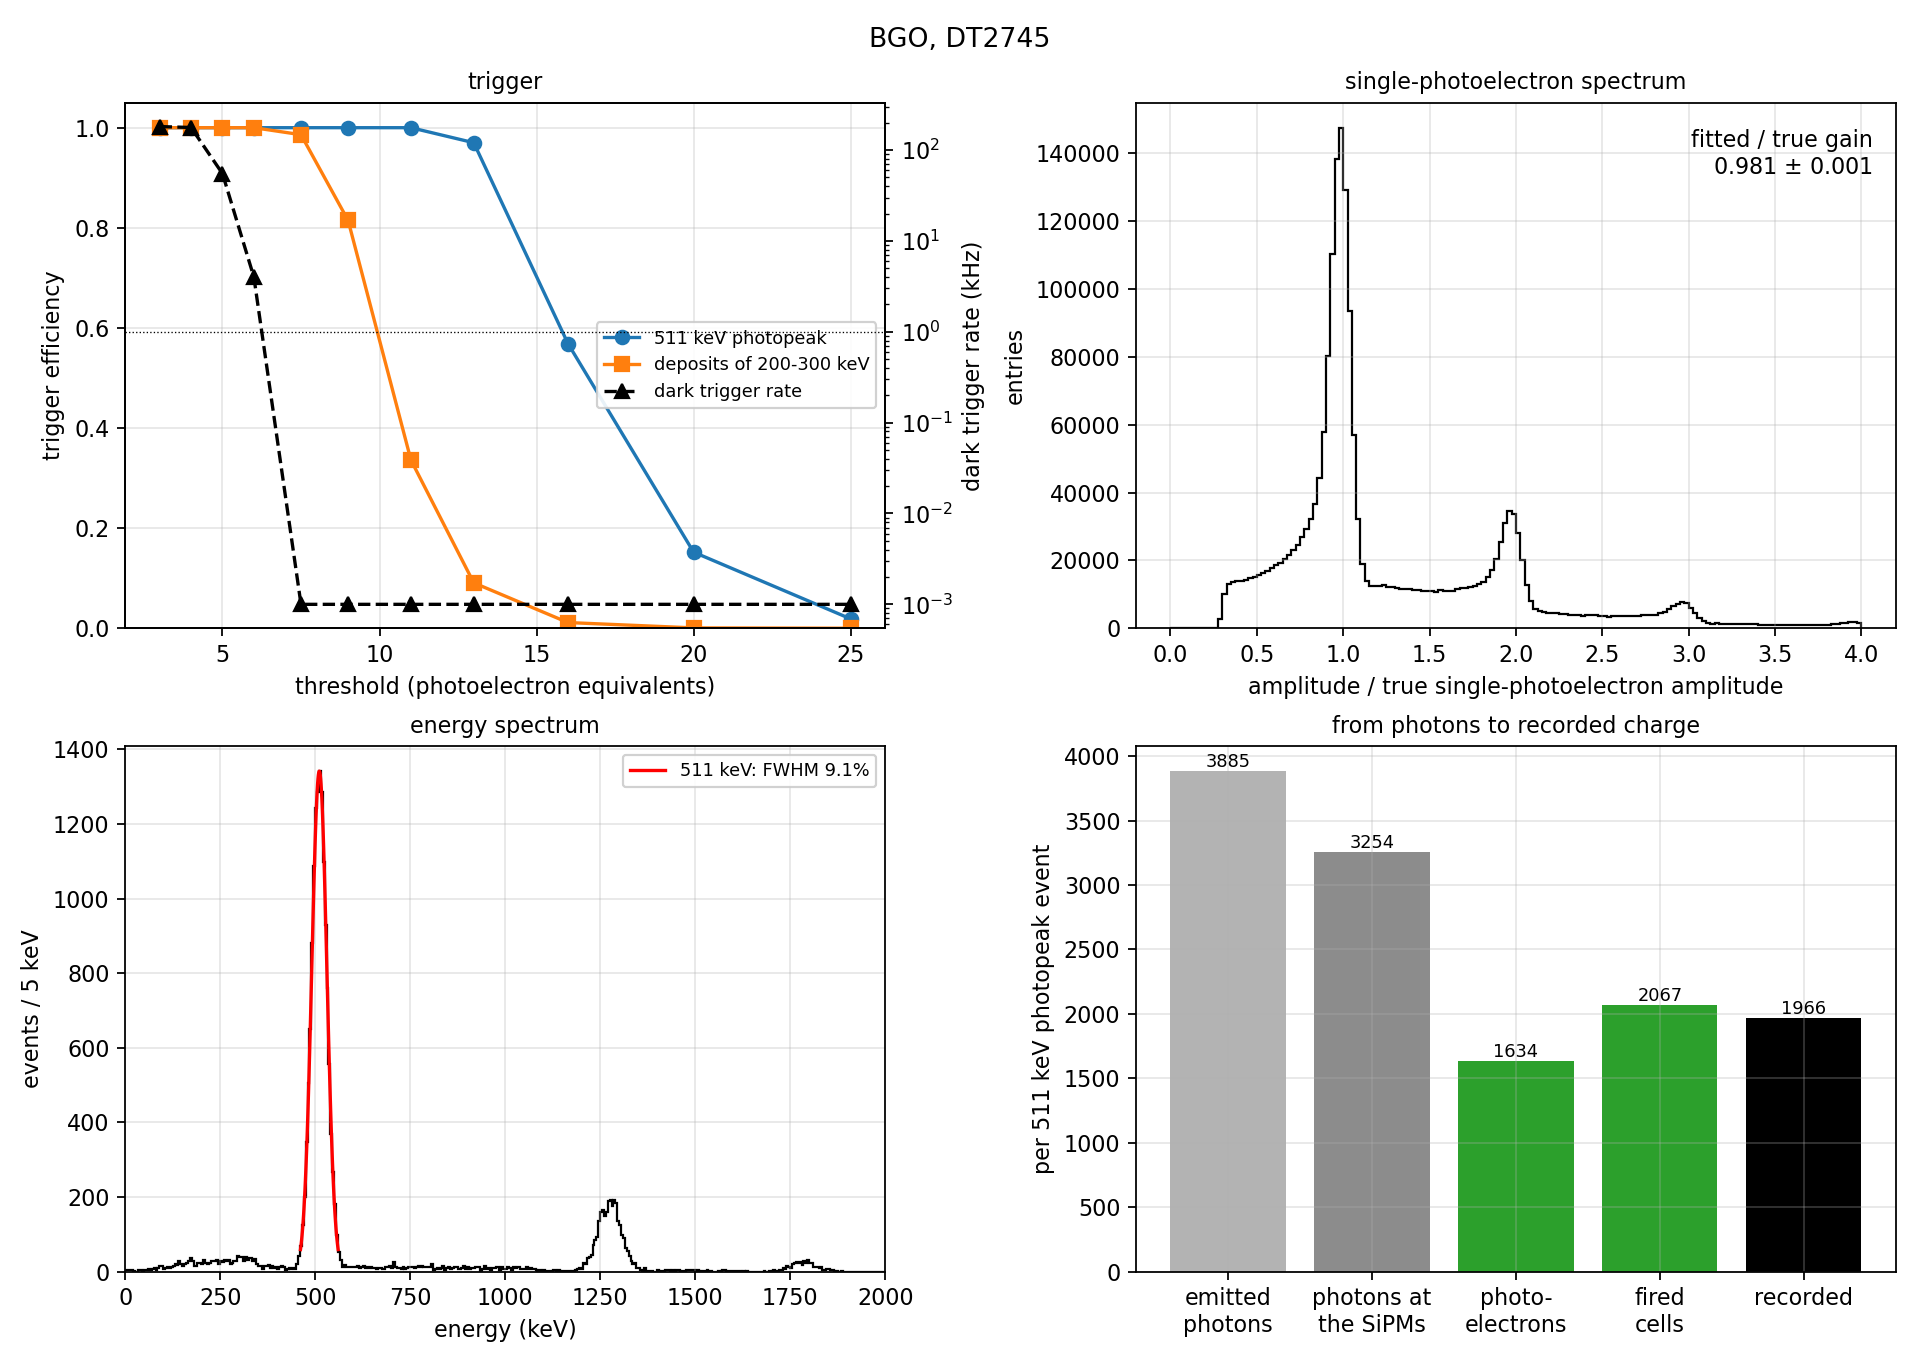
\includegraphics[width=\textwidth]{case_bgo_digitiser.png}
\caption{BGO read by the DT2745 digitiser at gain 4 and 5~V of
overvoltage. Panels as in Figure~\ref{fig:bgo_citiroc}; the
single-photoelectron spectrum is that of the matched-filter amplitudes.}
\label{fig:bgo_dig}
\end{figure}

\subsection{Radioroc2}

The charge trigger at 40 photoelectron equivalents triggers on every
511~keV event but only on 72\% of the deposits between 200 and 300~keV,
since it requires one channel above threshold, and the brightest channel
of such a deposit is often below it; dark counts do not trigger
(Figure~\ref{fig:bgo_rr}). At the shaping of 1.8~\us no
single-photoelectron peak exists: about eight dark counts fall within the
shaping time of each channel and their signals pile up. The calibration is
therefore taken at a peaking time of 300~ns, where the peaks are clean
and the fitted gain follows the true one to 1.4\%; the gain at 1.8~\us
follows from the ratio of the shaper gains at the two peaking times, which
the simulation knows exactly and the measurement must determine, for
instance with the charge-injection input of the chip. The long shaping
keeps almost all the light: the recorded charge, 1670 photoelectron
equivalents, is 1.05 times the photoelectrons. The pedestal is 785
photoelectron equivalents over the 64 channels; its subtraction leaves an
offset of 64~keV in the energy scale, and a ratio of the peak positions of
2.71, which the two-point calibration absorbs. The energy resolution is
8.5\% FWHM, with a readout contribution of 2.9\%.

\begin{figure}[htbp]
\centering
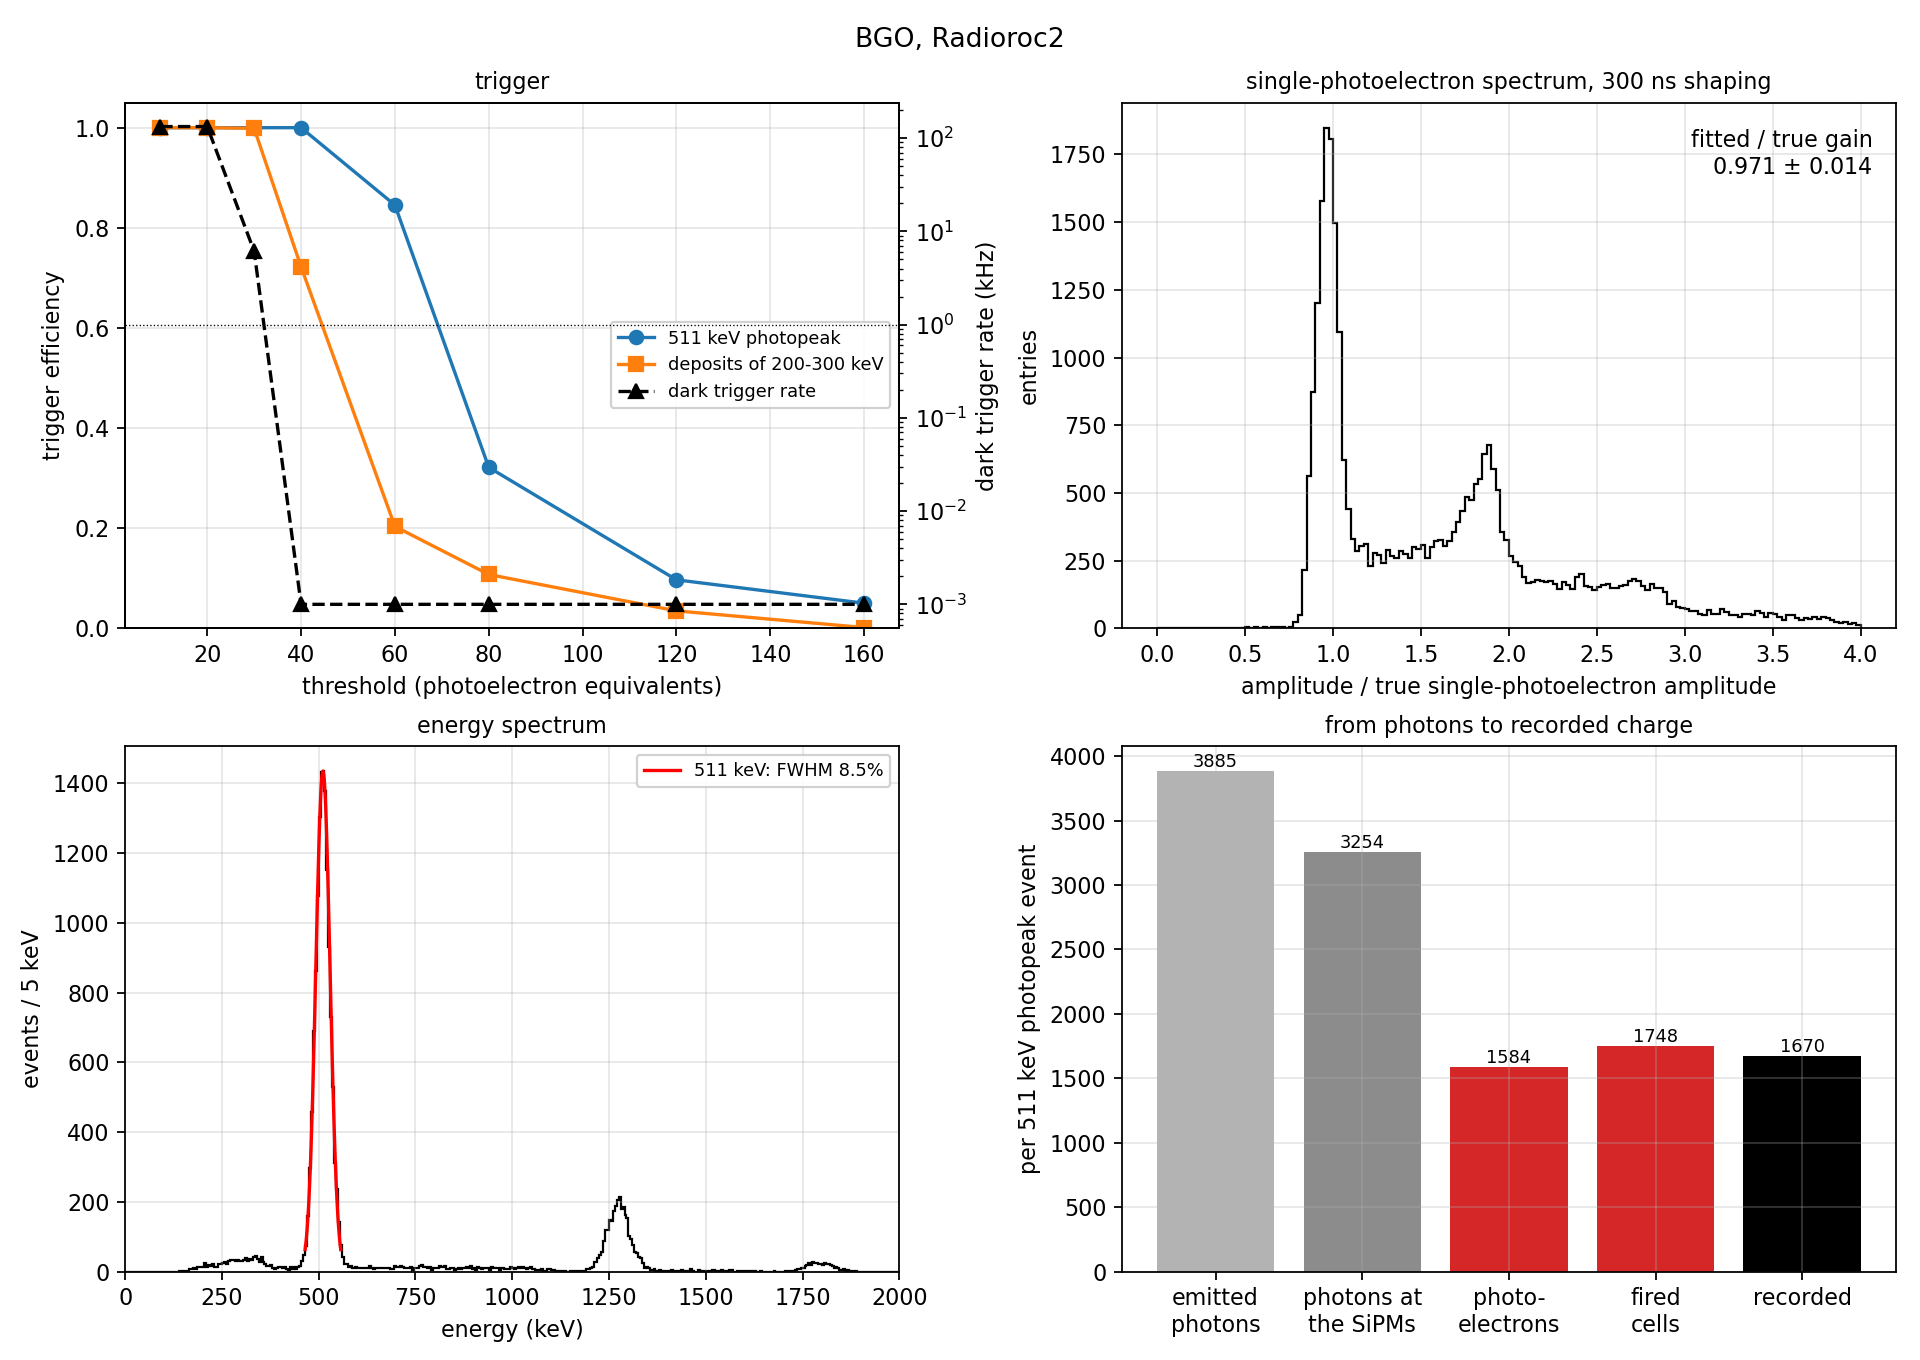
\includegraphics[width=\textwidth]{case_bgo_radioroc.png}
\caption{BGO read by the Radioroc2 at 1.8~\us of shaping. Panels as in
Figure~\ref{fig:bgo_citiroc}; the single-photoelectron spectrum is taken
at 300~ns of shaping.}
\label{fig:bgo_rr}
\end{figure}

\section{\csitl}
\label{sec:csi}

A 511~keV deposit in \csitl emits 27\,600 photons, of which 23\,210 (84\%)
reach the SiPMs. The detection efficiency at the 550~nm emission is lower
than at 480~nm, and the number of photoelectrons depends on the
overvoltage: 7215 at 2.0~V, 8820 at 2.7~V and 9523 at 5~V. The
statistical contribution to the width is therefore 2.4 to 3.0\%, half of
the intrinsic 5\%.

\subsection{Citiroc 1A}

The single-channel threshold of 7 photoelectron equivalents triggers on
every event of the two classes, at a dark trigger rate of 0.6~kHz
(Figure~\ref{fig:csi_citiroc}); the calibration is that of BGO, with a
fitted gain of 0.884 of the true one and a spread of 1.0\% between
channels. The shaping of 87.5~ns keeps a sixth of the photoelectrons of a
light pulse that lasts microseconds: the recorded charge is 1461
photoelectron equivalents, 0.17 of the 8820 photoelectrons. The energy
resolution is 7.4\% FWHM, of which the readout contributes 5.0\%, the
largest term. The brightest channel exceeds the input range of the chip in
3.4\% of the photopeak events; this saturation bends the response, with a
ratio of the peak positions of 2.44.

\begin{figure}[htbp]
\centering
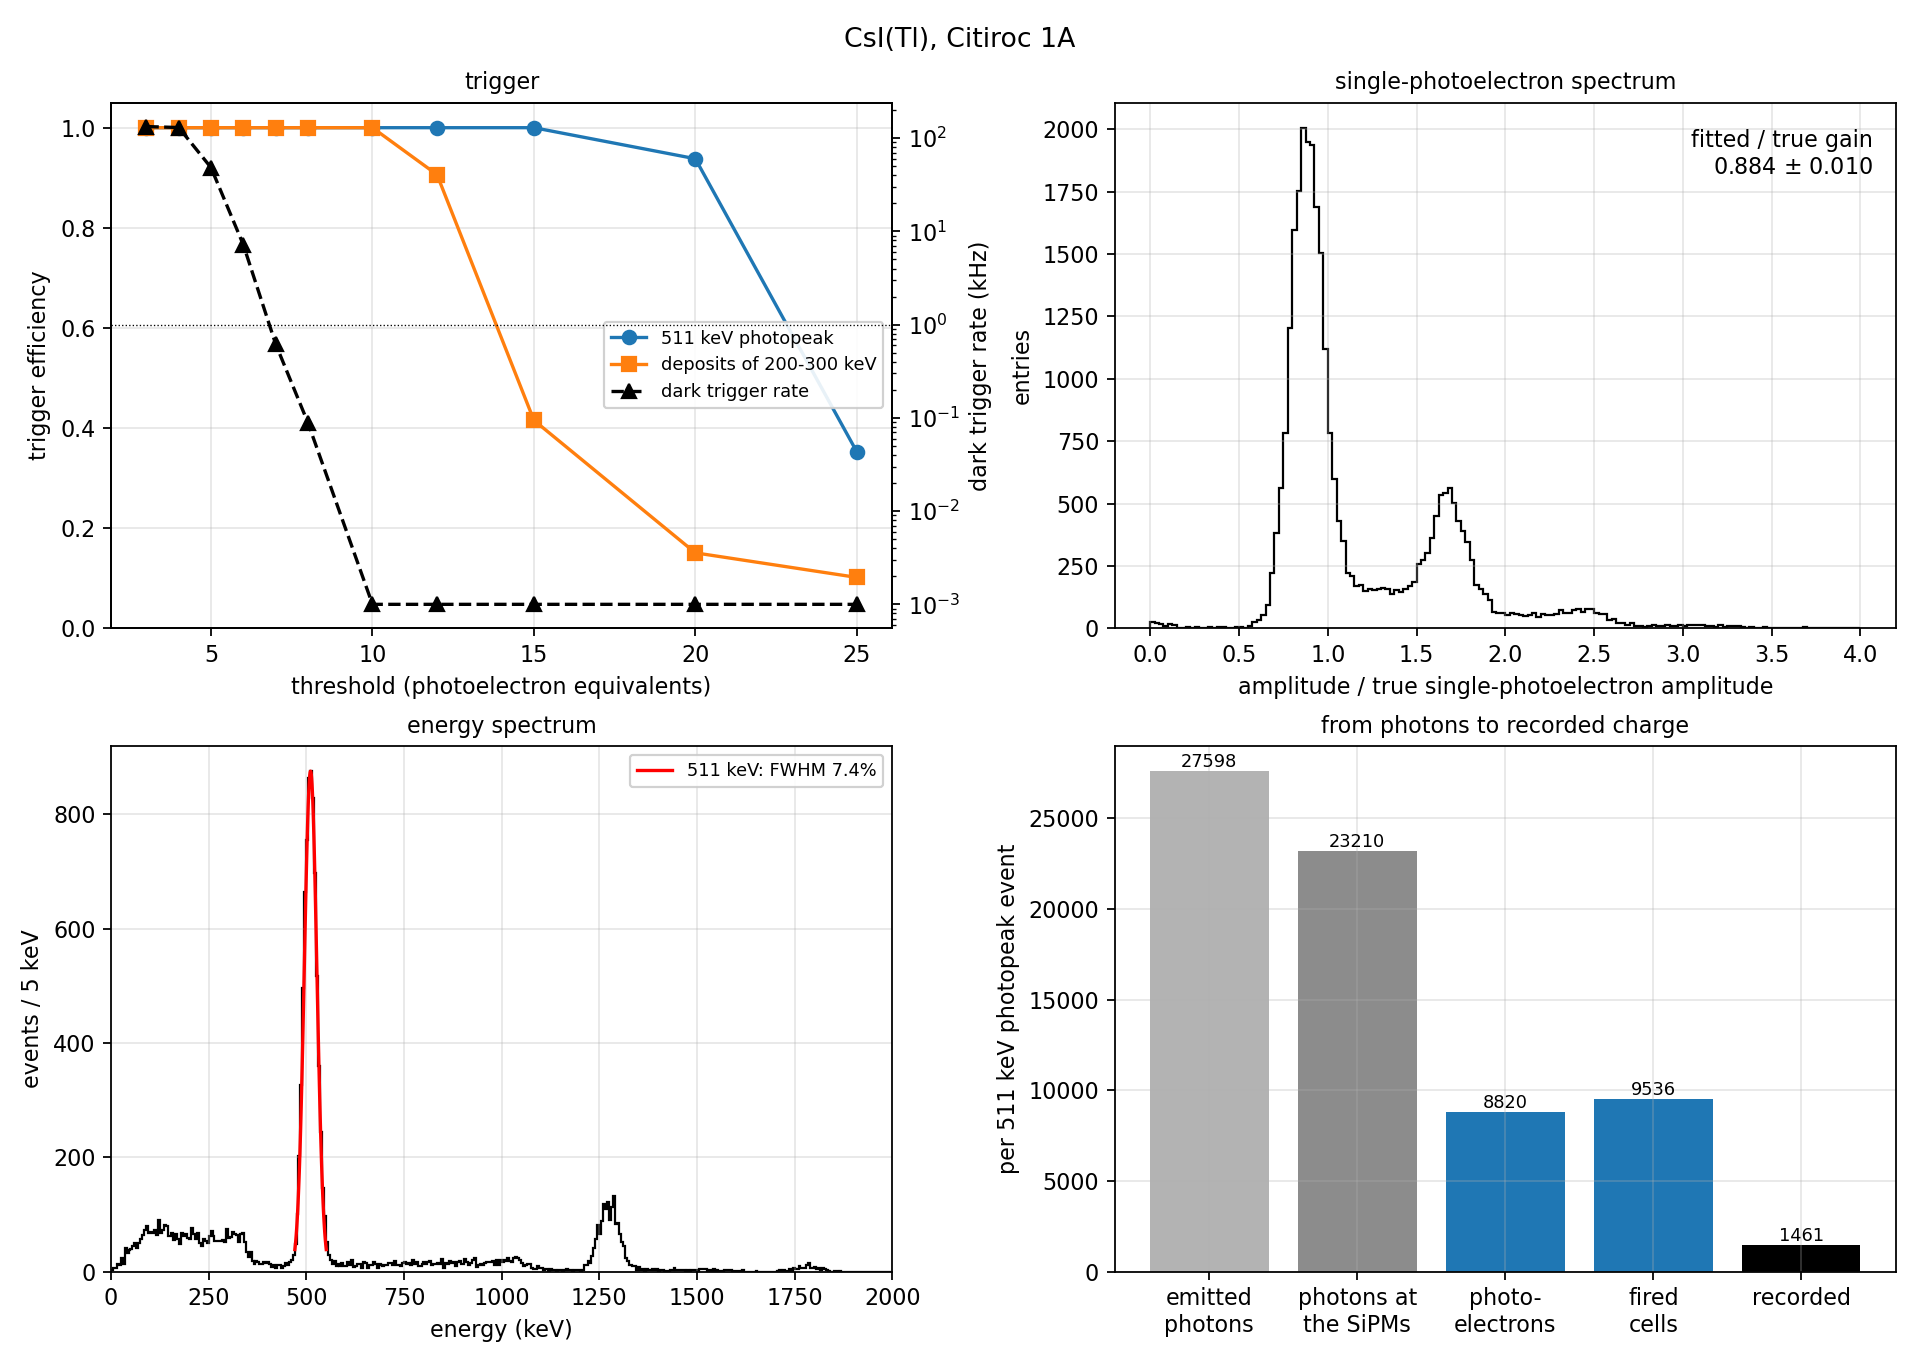
\includegraphics[width=\textwidth]{case_csitl_citiroc.png}
\caption{\csitl read by the Citiroc~1A. Panels as in
Figure~\ref{fig:bgo_citiroc}.}
\label{fig:csi_citiroc}
\end{figure}

\subsection{DT2745 digitiser}

The trigger and the calibration are those of BGO; every event of the two
classes triggers and no dark trigger occurs in the sample
(Figure~\ref{fig:csi_dig}). The integration window of 3~\us holds most of
both light components: the recorded charge is 10\,087 photoelectron
equivalents, 1.06 times the 9523 photoelectrons, the crosstalk compensating
the light that falls after the window. The energy resolution is 6.1\%
FWHM. The window collects 850 dark counts on average, and the readout
contributes 2.7\%; no channel saturates.

\begin{figure}[htbp]
\centering
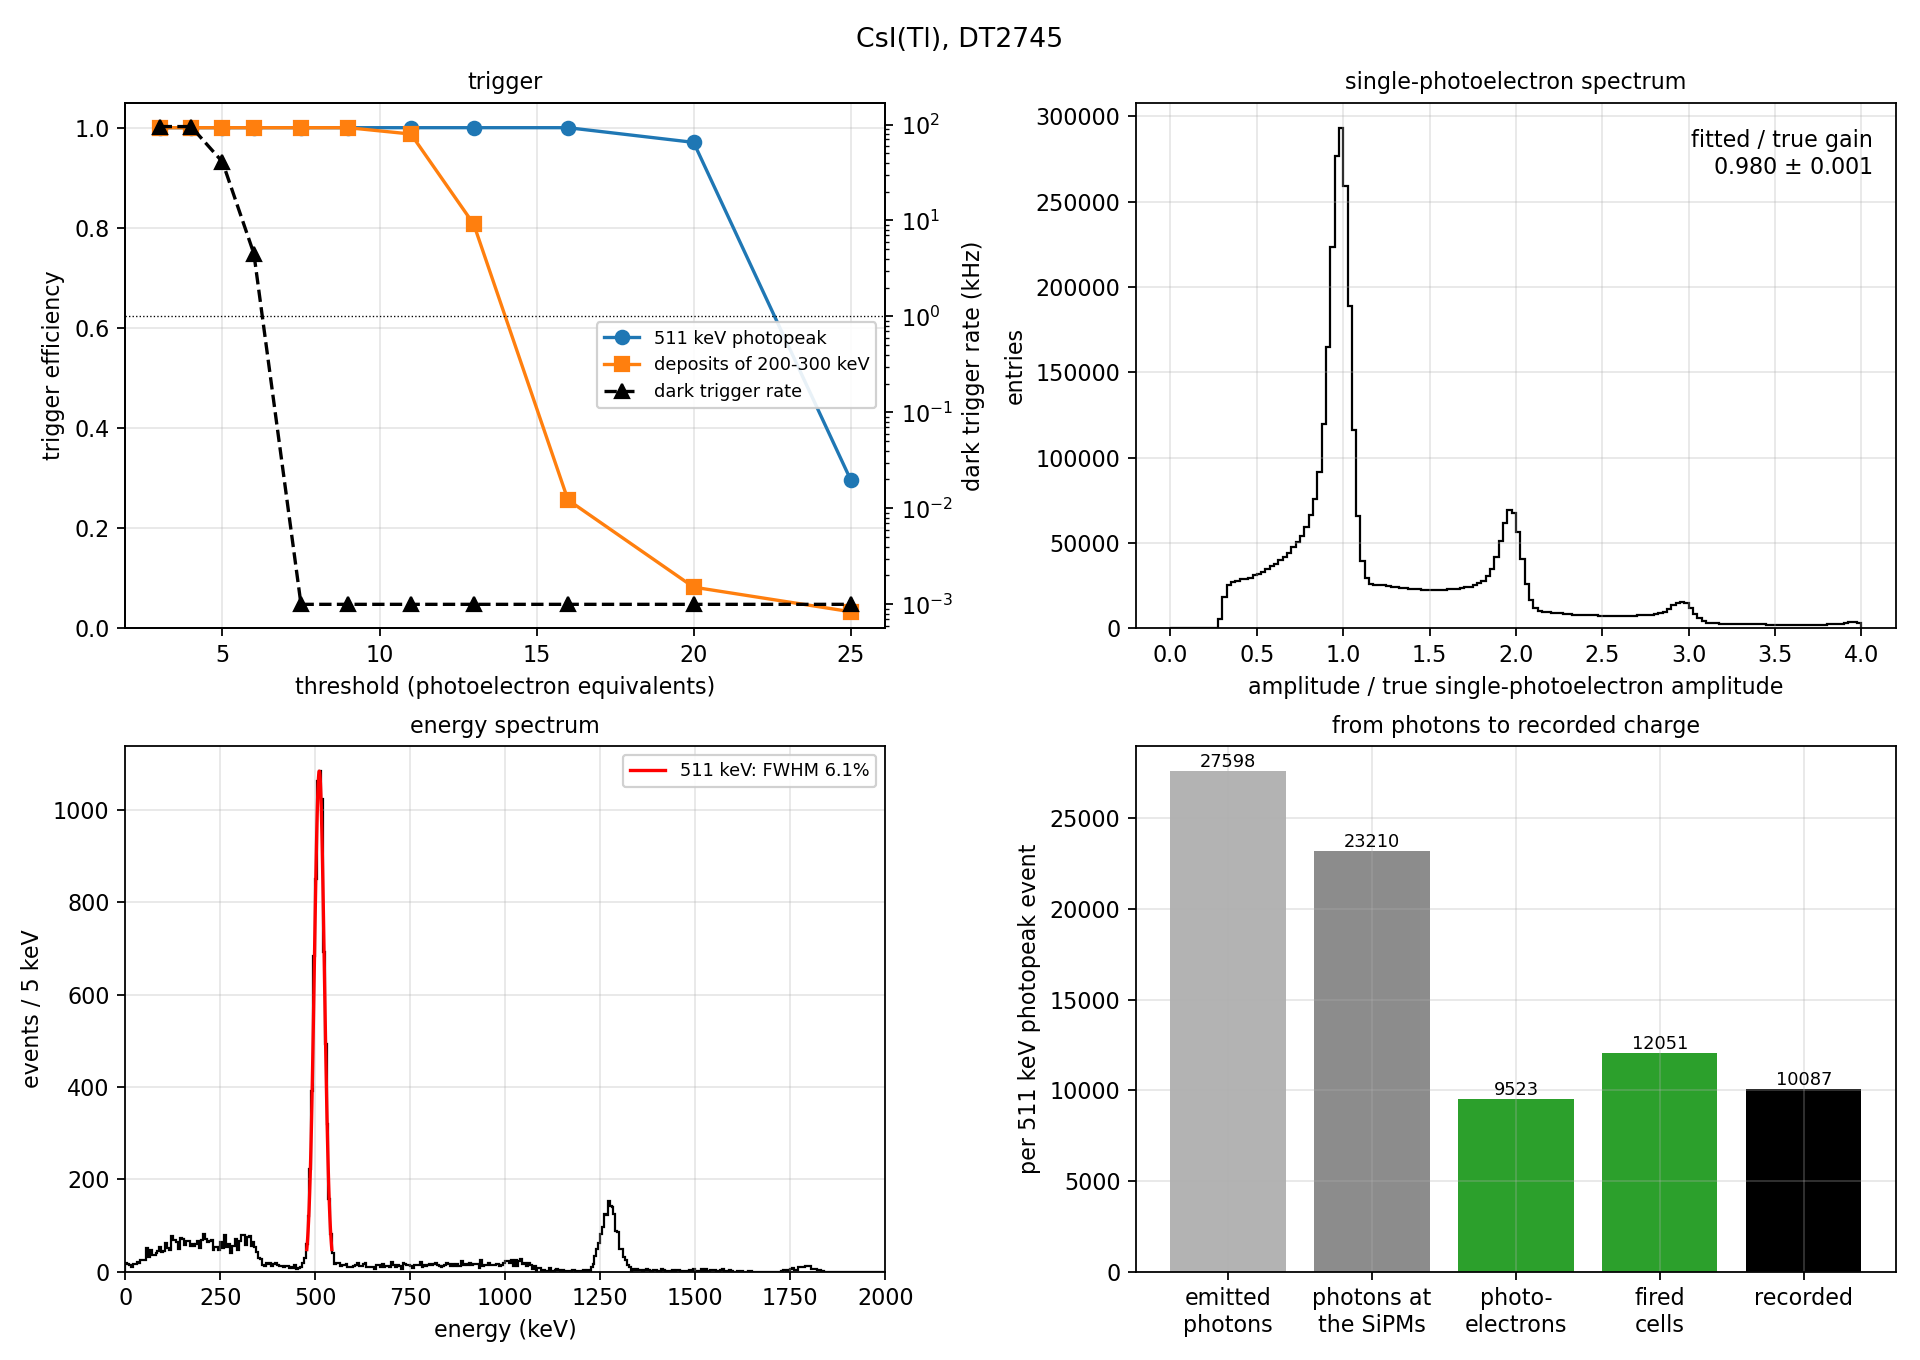
\includegraphics[width=\textwidth]{case_csitl_digitiser.png}
\caption{\csitl read by the DT2745 digitiser. Panels as in
Figure~\ref{fig:bgo_dig}.}
\label{fig:csi_dig}
\end{figure}

\subsection{Radioroc2}

The charge trigger at 40 photoelectron equivalents triggers on every event
of the two classes (Figure~\ref{fig:csi_rr}). The calibration at 300~ns
gives a fitted gain of 0.967 of the true one, with a spread of 1.5\%. At
2.0~V the brightest channel exceeds the low-gain range in 0.7\% of the
photopeak events, against at least 2.7\% at 2.7~V, at the price of 18\% fewer
photoelectrons than at 2.7~V. The shaping of 1.8~\us keeps 0.74 of the
photoelectrons, 5331 photoelectron equivalents. The energy resolution is
6.1\% FWHM, with a readout contribution of 1.8\%, the smallest of the six
cases; the ratio of the peak positions after the pedestal subtraction is
2.52.

\begin{figure}[htbp]
\centering
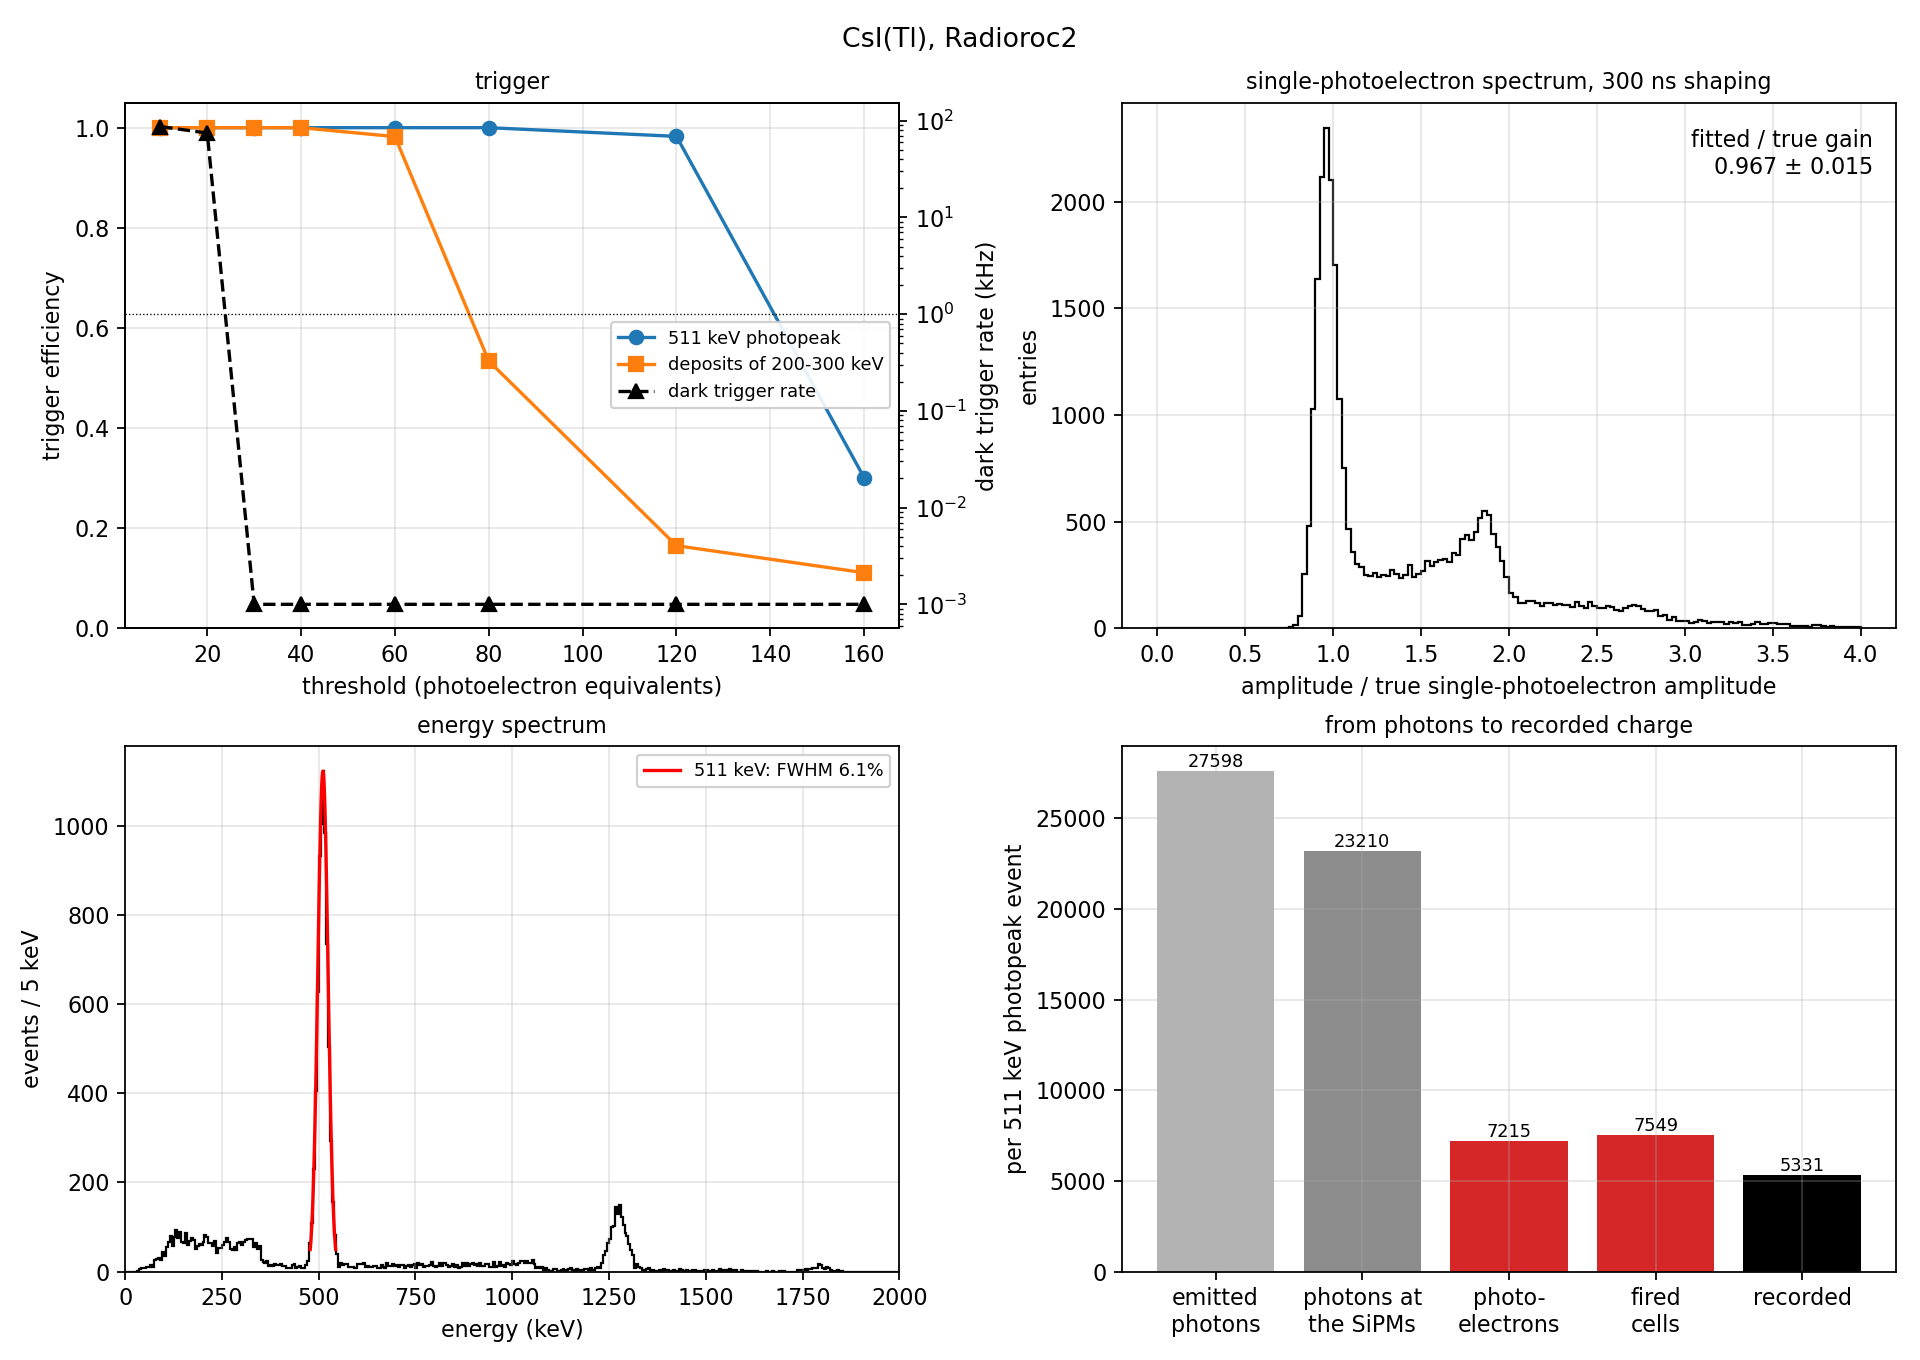
\includegraphics[width=\textwidth]{case_csitl_radioroc.png}
\caption{\csitl read by the Radioroc2. Panels as in
Figure~\ref{fig:bgo_rr}.}
\label{fig:csi_rr}
\end{figure}

\section{Comparison}
\label{sec:comparison}

Figure~\ref{fig:resolution} gathers the energy resolutions and their
decomposition. For BGO the three readouts span 8.5 to 10.1\%, for \csitl
6.1 to 7.4\%, and in every case the intrinsic resolution of the crystal
and the statistics of the photoelectrons account for most of the width.
For BGO the statistical term, 5.9\%, is as large as the intrinsic one,
because the crystal produces few photons; for \csitl it is half of it.
The readout term orders the three readouts in the same way for both
crystals: it is largest for the Citiroc, whose shaping of 87.5~ns records
a fluctuating fraction of a long light pulse; intermediate for the
digitiser, whose integration window collects dark counts in proportion to
its length; and smallest for the Radioroc2, whose 1.8~\us shaping records
nearly all the light. The digitiser pays in
addition for the 19.5\% crosstalk of the 5~V overvoltage at which it
operates. With BGO, the digitiser at 3~V of overvoltage, where the
crosstalk is 9\%, reaches 8.8\% in the same simulation; with \csitl it
makes no difference.

\begin{figure}[htbp]
\centering
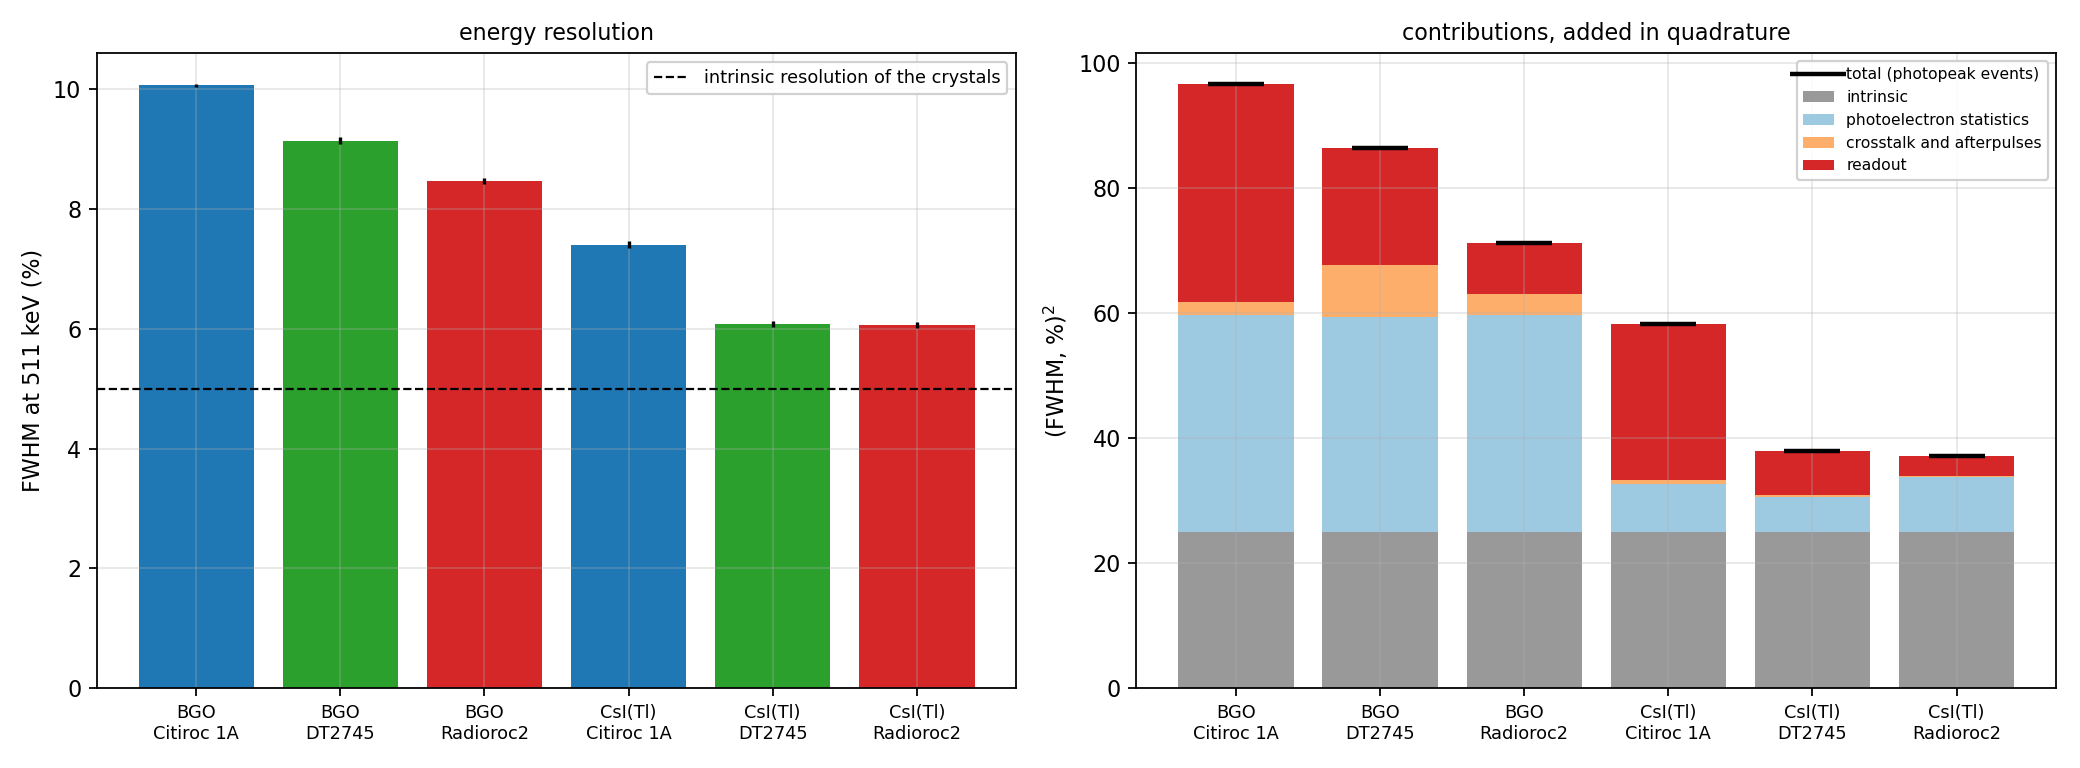
\includegraphics[width=\textwidth]{compare_resolution.png}
\caption{Left: energy resolution at 511~keV of the six cases, with the
intrinsic resolution of the crystals. Right: the squares of the
contributions to the width of the photopeak events, stacked; the bar marks
the total.}
\label{fig:resolution}
\end{figure}

Figure~\ref{fig:light} shows the chain from photons to recorded charge.
The collection efficiency, 0.84, is a property of the crystal and its
coupling and is common to the three readouts. The detection efficiency at
the emission wavelength is 0.49 to 0.50 for BGO and 0.31 to
0.41 for \csitl, depending on the overvoltage. The fraction of the
photoelectrons recorded spans an order of magnitude: 0.17 for \csitl and
0.46 for BGO with the Citiroc, close to one with the Radioroc2 and above
one with the digitiser, whose integral includes the crosstalk. The number
of photoelectrons sets the statistical limit; the recorded fraction sets
how close a readout comes to it.

\begin{figure}[htbp]
\centering
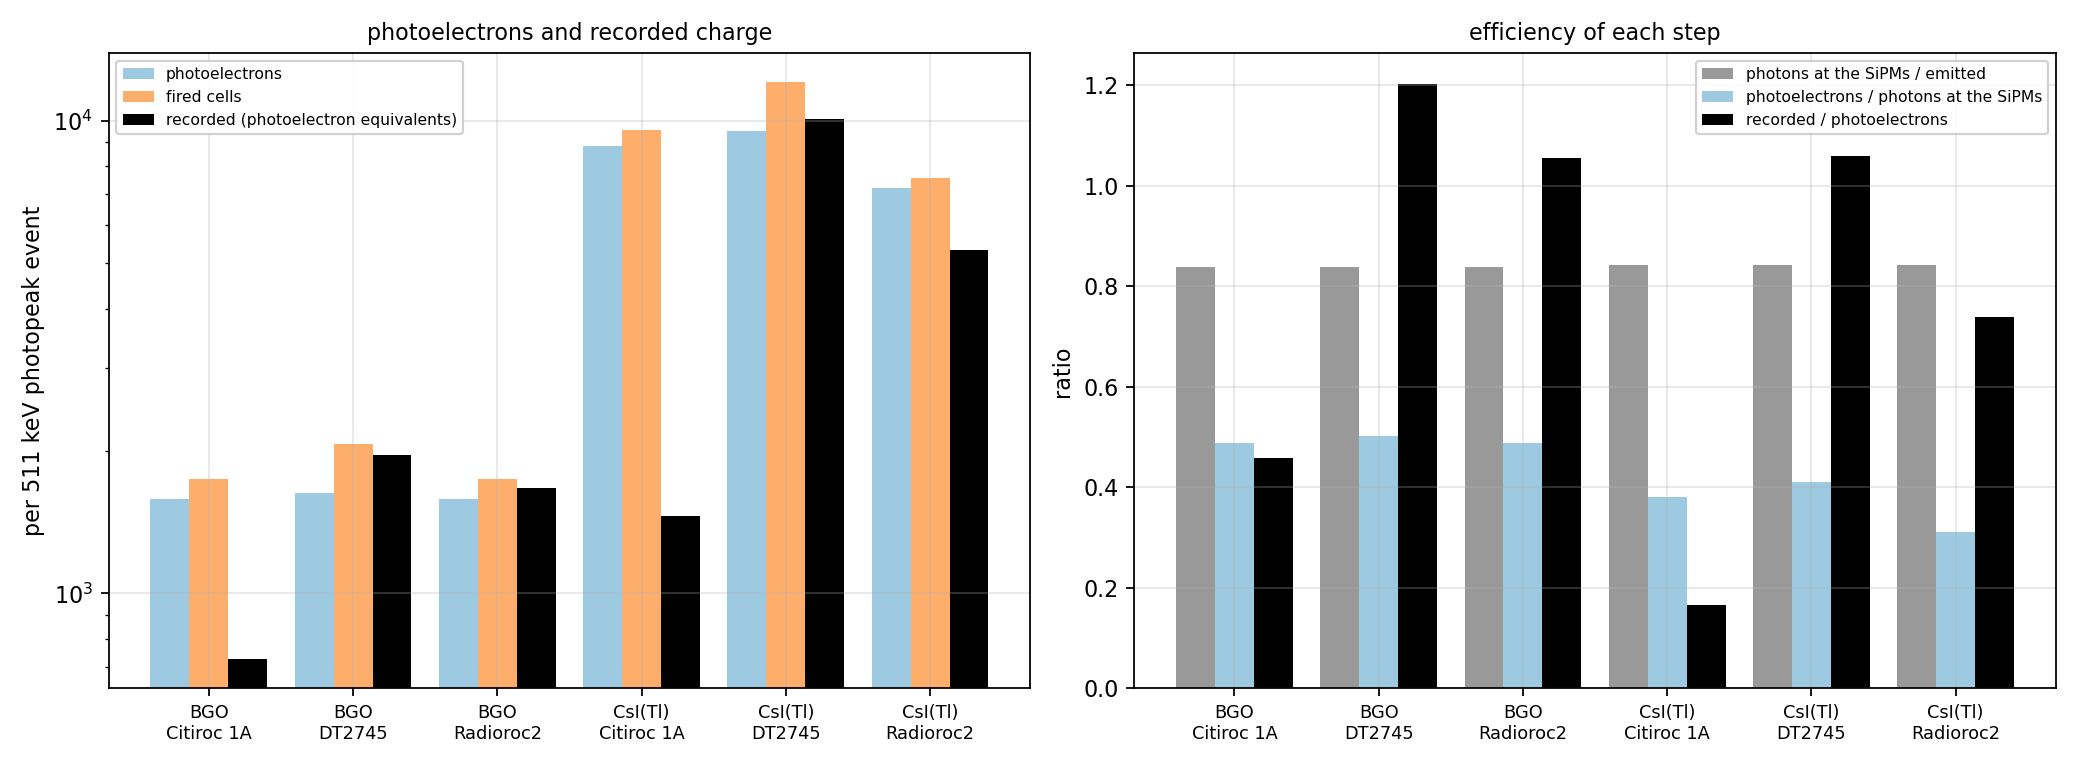
\includegraphics[width=\textwidth]{compare_light.png}
\caption{Left: photoelectrons, fired cells and recorded charge per 511~keV
photopeak event. Right: collection efficiency, detection efficiency and
fraction of the photoelectrons recorded.}
\label{fig:light}
\end{figure}

Figure~\ref{fig:channels} shows the distributions of the brightest and of
the least illuminated channel in the photopeak events, the two ends of the
dynamic range that a position measurement needs. In BGO the brightest
channel holds a median of 29 photoelectron equivalents with the Citiroc,
58 with the Radioroc2 and 74 with the digitiser, and the least illuminated
one 3 to 9; in \csitl the brightest channel reaches 1800 photoelectron
equivalents in one event of a hundred with the digitiser, which its range
holds, and 940 with the Radioroc2, at the limit of its low gain.

\begin{figure}[htbp]
\centering
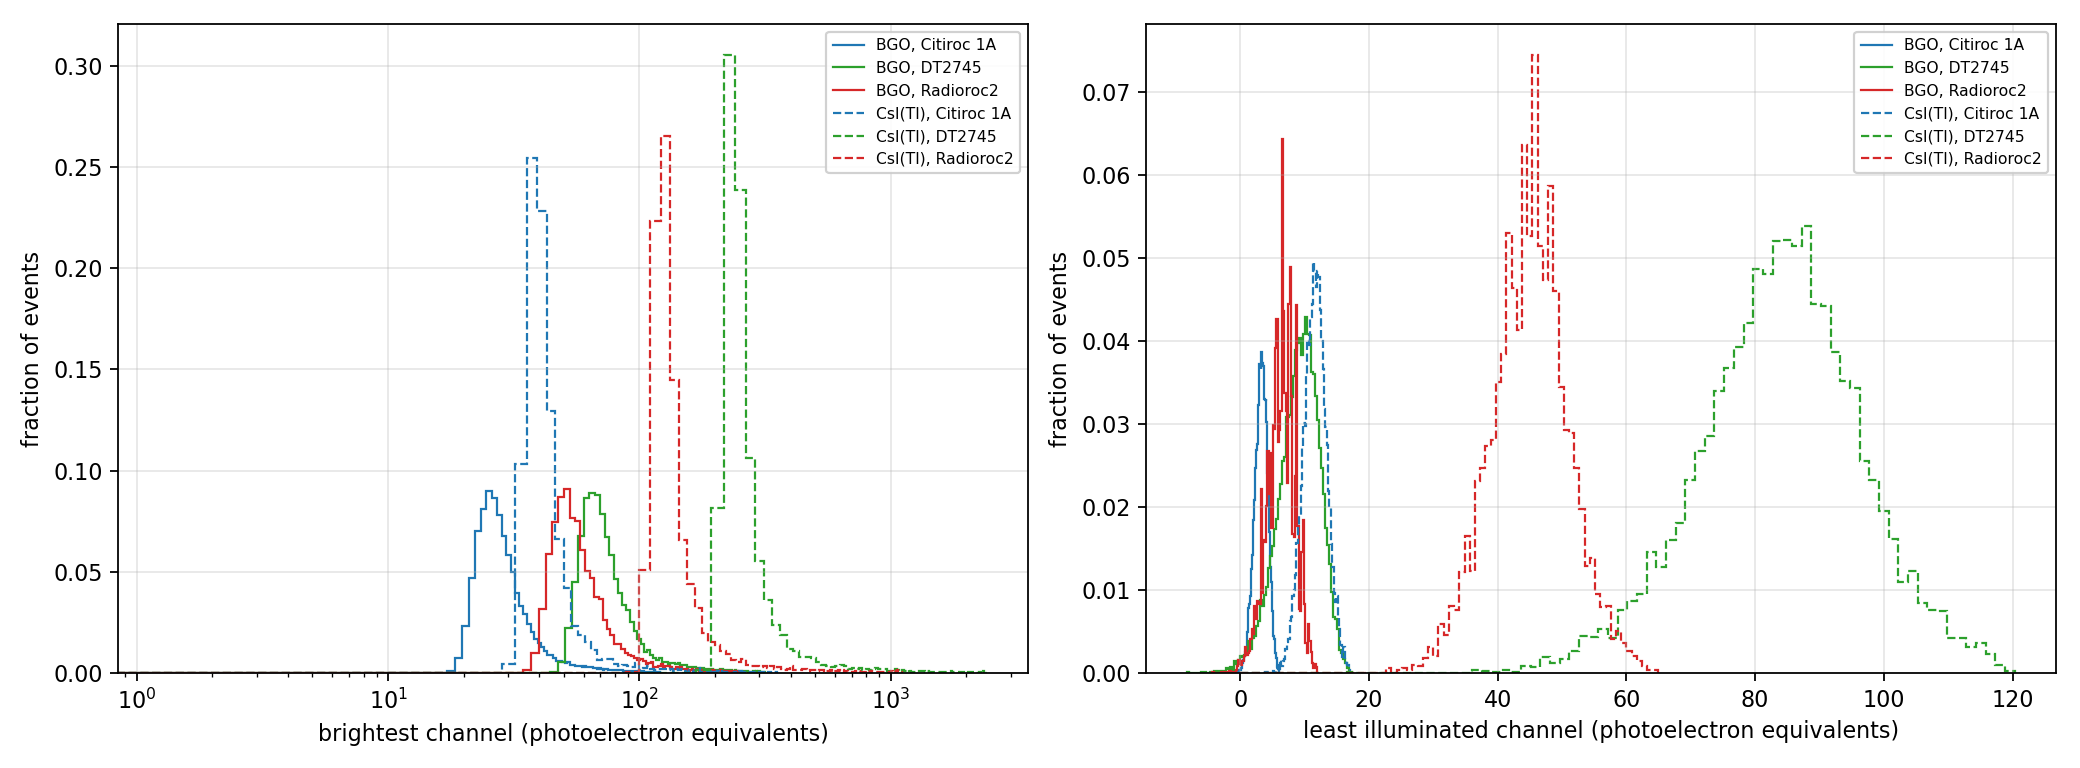
\includegraphics[width=\textwidth]{compare_channels.png}
\caption{Brightest (left) and least illuminated (right) channel of the
511~keV photopeak events, pedestal subtracted, in photoelectron
equivalents. Solid lines BGO, dashed lines \csitl.}
\label{fig:channels}
\end{figure}

\section{Conclusions}
\label{sec:conclusions}

At room temperature the three readouts measure the energy of a 511~keV
deposit with resolutions within 1.6 points of each other for BGO and
1.3 points for \csitl. The resolution is limited by the crystal, through
its intrinsic resolution and, for BGO, its low light yield; the readout
adds a term that ranges from 5 to 6\% FWHM for the Citiroc down to 2 to
3\% for the Radioroc2. The dark counts of the SiPMs, about 4~MHz per
channel, shape the operation of every readout: they set the trigger
thresholds at 7 to 8 photoelectrons, add to the width through the
integration window of the digitiser and the pedestal of the peak
detectors, and determine how the gain can be calibrated. The digitiser
must run at gain 4, at which its single-photoelectron peaks are
separated, and analyse its records with a matched filter; the Radioroc2
must be calibrated at a short shaping time and transfer the gain to its
long one; the Citiroc calibrates directly. The measurements of the coming
weeks will test these predictions, starting with the number of
photoelectrons and the single-photoelectron spectra, which are the least
dependent on the readout.

\end{document}
